% ----------------------- TODO ---------------------------
% Diese Daten müssen pro Blatt angepasst werden:
\newcommand{\NUMBER}{2}
\newcommand{\EXERCISES}{5}
% Diese Daten müssen einmalig pro Vorlesung angepasst werden:
\newcommand{\COURSE}{Grundlagen der Digitaltechnik}
\newcommand{\TOPIC}{ALU}
\newcommand{\DATE}{29.04.2022}
% ----------------------- TODO ---------------------------

\documentclass[a4paper]{scrartcl}

\usepackage[utf8]{inputenc}
\usepackage[ngerman]{babel}
\usepackage{amsmath}
\usepackage{amssymb}
\usepackage{fancyhdr}
\usepackage{color}
\usepackage{graphicx}
\usepackage{lastpage}
\usepackage{listings}
\usepackage{tikz}
\usepackage{pdflscape}
\usepackage{subfigure}
\usepackage{float}
\usepackage{polynom}
\usepackage{hyperref}
\usepackage{tabularx}
\usepackage{forloop}
\usepackage{geometry}
\usepackage{listings}
\usepackage{fancybox}
\usepackage{tikz}
\usepackage{algpseudocode,algorithm,algorithmicx}

%Definiere Let-Command für algorithmen
\newcommand*\Let[2]{\State #1 $\gets$ #2}

\input kvmacros

%Größe der Ränder setzen
\geometry{a4paper,left=3cm, right=3cm, top=3cm, bottom=3cm}

%Kopf- und Fußzeile
\pagestyle {fancy}
\fancyhead[L]{\COURSE}
\fancyhead[R]{\DATE}

\fancyfoot[L]{}
\fancyfoot[C]{}
\fancyfoot[R]{Seite \thepage /\pageref*{LastPage}}
\setlength{\parindent}{0pt}

%Formatierung der Überschrift, hier nichts ändern
\def\header#1#2{
  \begin{center}
    {\Large Labor #1: \TOPIC}\\
    {(Datum #2)}
  \end{center}
}


\begin{document}


\header{Nr. \NUMBER}{\DATE}



% ----------------------- TODO ---------------------------
% Hier werden die Aufgaben/Lösungen eingetragen:
\section*{Aufgabe 1: Simulieren einer ALU}
Der unten abgedruckte Aufbau einer ALU ist auch in Kapitel 5 auf Slide ``ALU III'' zu sehen. Diese ALU soll in Logisim mit 8-Bit Registerbreite
nachgebaut werden. 
% \begin{center}
  
\begin{figure}[h]
  \centering
    \includegraphics[width=8cm]{../../Slides/Images/SimpleALU.png}
  \end{figure}
% \end{center}

\subsection*{a) Building Blocks}
Um die ganze Schaltung übersichtlicher zu gestalten, sollten die verschiedenen Blöcke der Schaltung als jeweils eigenes 
Subsystem implementiert werden. Lege daher für die Blöcke:
\begin{itemize}
  \item Inverter
  \item Gate
  \item AND
  \item OR
  \item XOR
  \item Adder 
\end{itemize}

jeweils ein eigenes Subsystem an. Bedenke die 8-Bit Registerbreite.

\textbf{Hinweise:}
\begin{itemize}
  \item Um die Verbindungen übersichtlicher zu machen, können Splitter verwendet werden.
  \item Die logischen Operationen (AND, OR, XOR) arbeiten auf Bit-Ebene  
  \begin{itemize}
    \item vgl. Bitwise-OR (-AND) in C ($\vert$, \&)
    \item Bsp. A = 0xAA, B = 0x55 $\rightarrow$ A AND B = 0x00
  \end{itemize}
  \item Adder:
  \begin{itemize}
    \item Es empfielt sich weitere Subsysteme anzulegen (z.B. 1-Bit-Fulladder)
    \item Bedenke, dass der unterste Carry-In auch mit rausgeführt werden muss (die einer Stelle)
    \item Für unsere Zwecke ist der Addierer von der Slide ``Volladdierer II'' ausreichend, ein Carry-Look-Ahead Addierer wird nicht benötigt 
  \end{itemize}
  \item Funktion des Gate-Blocks: Wenn Enable=1, dann Output=B, sonst Output=0x00 
  \item Funktion des Inverter-Blocks: Wenn Invert=1, dann Output=$\overline{A}$, sonst Output=$A$
  \begin{itemize}
    \item Auch der Inverter arbeitet auf Bit-Ebene
  \end{itemize}
\end{itemize}

\subsection*{b) Unit Tests}
Jetzt wurden die grundlegenden Funktionsblöcke für die ALU erstellt. Diese sollen nun einzeln auf korrekte Funktionalität getestet werden.
Daher soll für jeden der erstellten Blöcke eine Testschaltung angelegt werden. Nenne diese \textit{Test\_$<$Blockname$>$}.
Dort soll jeweils der Block eingefügt werden und die Ein- und Ausgänge des Blocks beschalten werden. Überprüfe in der Simulation 
die korrekte Funktionalität

\begin{figure}[h]
  \centering
  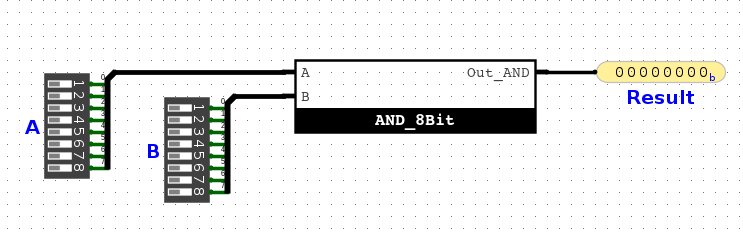
\includegraphics[width=12cm]{Test_Circuit.png}
\end{figure}

\subsection*{c) Erstellen der ALU}
Nachdem Test sollten jetzt alle Blöcke ihre korrekte Funktion besitzen. Lege nun ein weiteres Subsystem für die ALU an z.B. ``ALU\_8Bit''. 
Baue nach dem Bild auf Seite 1 die ALU zusammen.\\
\begin{itemize}
  \item Für den Multiplexer kann der von Logisim bereitgestellte Multiplexer benutzt werden. Mit Select-Bits wählt man die Anzahl der Steuereingänge und
  damit auch die Anzahl der Dateneingänge. Mit Data-Bits wählt man die breite der einzelnen Dateneingänge und des Ausgangs.
  \item Das fertige System soll 3 Eingänge besitzen F (4 Bit), A (8 Bit) und B (8 Bit)
  \item Es soll außerdem 2 Ausgänge R (8 Bit) und D (1 Bit) besitzen

\end{itemize}

\subsection*{d) Test der ALU}
Benutze den ``main'' Tab oder lege ein ``Test\_ALU'' Subsystem an, um die Funktionalität der ALU zu testen. Gehe hier gleich vor wie bei den 
Unit Tests aus Aufgabenteil b).\\

Nachdem die Funktion der ALU nun verifiziert wurde und diese funkitioniert kann in die Tabelle am Ende nun eingetragen werden, was die ALU für
die verschiedenen Zustände des Funktionsregisters F durchführt.
\begin{itemize}
  \item Sind alle Zustände von F sinnvoll?
  \item Was zeigt das Ausgangsbit D an?
\end{itemize}



\subsection*{d) Flags (Bonus)}
ALUs werden in CPU Kernen benutzt. Die CPU Kerne besitzen meist ein ``Flags'' Register, welches verschiedene Zustände der letzten
Operation der ALU anzeigt. Diese werden von der ALU ausgegeben und dann in einem Register gespeichert.
In dem aktuellen Design geben wir im Output D ein einziges ``Flag'' aus, das Carry-Flag. 
Dieses zeigt an, ob es beim Rechnen einen Übertrag im MSB (most significant bit) gab. Erweitere die ALU so, dass D auch noch folgende zusätzliche 
Flags ausgibt:
\begin{itemize}
  \item Zero-Flag: Zeigt an, ob das Ergebnis der letzten Operation 0 war
  \item Overflow-Flag: Zeigt an, ob es beim Rechnen mit Zahlen im 2er Komplement einen Overflow gab (s. Slide ``Subtrahierer I'' und ``Subtrahierer II'')
  \item Sign-Flag: Wenn das letzte Ergebnis negativ war Flag = 1, sonst 0
  \item Parity-Flag: Zeigt die Parität des letzten Ergebnisses an. Odd = 0, Even = 1
\end{itemize}


\newpage
\begin{table}
  \LARGE
  \centering
  \begin{tabular}[h]{c|cccc|c}
    \multicolumn{5}{c|}{\textbf{Wert von F}} & \textbf{Funktion} \\ \hline
    Hex & $F_3$ & $F_2$ & $F_1$ & $F_0$ & $<$Funktionstext z.B. R = A + B$>$\\\hline
    0x0 & 0 & 0 & 0 & 0 & \\\hline 
    0x1 & 0 & 0 & 0 & 1 & \\\hline 
    0x2 & 0 & 0 & 1 & 0 & \\\hline 
    0x3 & 0 & 0 & 1 & 1 & \\\hline 
    0x4 & 0 & 1 & 0 & 0 & \\\hline 
    0x5 & 0 & 1 & 0 & 1 & \\\hline 
    0x6 & 0 & 1 & 1 & 0 & \\\hline 
    0x7 & 0 & 1 & 1 & 1 & \\\hline 
    0x8 & 1 & 0 & 0 & 0 & \\\hline 
    0x9 & 1 & 0 & 0 & 1 & \\\hline 
    0xA & 1 & 0 & 1 & 0 & \\\hline 
    0xB & 1 & 0 & 1 & 1 & \\\hline 
    0xC & 1 & 1 & 0 & 0 & \\\hline 
    0xD & 1 & 1 & 0 & 1 & \\\hline 
    0xE & 1 & 1 & 1 & 0 & \\\hline 
    0xF & 1 & 1 & 1 & 1 & \\ 
    
  \end{tabular}
\end{table}



  
\end{document}
%%% Local Variables:
%%% mode: latex
%%% TeX-master: t
%%% End: